\documentclass{beamer}
\usetheme{CENIDETDIE}
\setbeamertemplate{caption}[numbered]
\usefonttheme[onlymath]{serif}

% ------------------------------------------------------------------------------------------------

\usepackage[utf8]{inputenc}
\usepackage[T1]{fontenc}
\usepackage{helvet}
\usepackage{graphicx} % Allows including images
\usepackage{booktabs} % Allows the use of \toprule, \midrule and \bottomrule tables
\usepackage{amsmath}
\usepackage{color}
\usepackage{hyperref}
\usepackage{subfig}
\usepackage[document]{ragged2e}
%\usepackage{authblk} %many authors
\numberwithin{figure}{section}
%\numberwithin{equation}{section}
\usepackage{natbib}
\usepackage{multirow}

% ------------------------------------------------------------------------------------------------

\title{\textbf{ \textit{W+jets to Leptons}}}
%\subtitle{{\small }}
\author[C.Salazar]{\textbf{Camilo A Salazar G} }
\institute[UdeA]{camilo.salazar@cern.ch}

%\author{\textit{\textbf{Camilo A Salazar G}}}
%\institute{\url{camilo.salazar@cern.ch} }
\date{\today}


% ------------------------------------------------------------------------------------------------

\begin{document}

% ------------------------------------------------------------------------------------------------

\begin{frame}[plain,t]
\titlepage
\end{frame}


% ------------------------------------------------------------------------------------------------

\begin{frame}[plain,noframenumbering]
  \addtocounter{framenumber}{-1}
  \scriptsize
%   \thispagestyle{empty}
  \frametitle{Contenido}
  \setbeamertemplate{section in toc}[sections numbered]
  \tableofcontents[hideallsubsections]
\end{frame}

% ------------------------------------------------------------------------------------------------

\section{Introduccion}
\begin{frame}
\frametitle{Introducción}
\justifying{Hay diferencia de opiniones respecto a dos cosas:}


\begin{itemize}
	\item[-] Las Secciones Eficazes que se están tomando para los diferentes Backgrounds (BG).
	\item[-] Para el Background principal, cuales son los estados fianles de interes.
	\begin{itemize}
		\item $W+jets$ con $W \rightarrow \mu \nu_{\mu}$
		\item $W+jets$ con $W \rightarrow \tau \nu_{\tau}$
	\end{itemize}
\end{itemize} 

\end{frame}

% -------------------------------------------------------------

\section{Secciones Eficazes}
\begin{frame}
\frametitle{Secciones Eficazes}

\begin{exampleblock}{Para W+Jest se tomó XS=3091.50 pb }
	\begin{itemize}
		\item Los resultados de Nelson Muestran 
		\begin{itemize}
			\item[]	Integrated weight (pb)          :  3601.38728785
			\item[] Matched Integrated weight (pb)  :  808.87158775
		\end{itemize} 					 
		\item La XS de las muestras oficiales de CMS de W+jets a los leptones del SM es 3781.881814 pb
	\end{itemize} 
	Cual usar y porque?
\end{exampleblock}

\end{frame}


% ----------------------------------------------------------------


\section{Uso del BG the Taus}
\begin{frame}
\frametitle{Uso del BG the Taus}
Le pregunte a la gente de MUONRECO, si experimentalmente se puede distinguir entre $W \rightarrow \mu \nu_{\mu}$ y $W \rightarrow \tau \nu_{\tau} \rightarrow \mu \nu_{\mu}$
\begin{exampleblock}{Me rospondio Dmytro Kovalskyi:}

Que en la region de bajo pT se debia hacer una estimación con montecarlo.

\end{exampleblock}

\begin{itemize}
	\item "A tight muon must be compatible with the primary vertex, having a transverse impact parameter |dXY| < 0.2 cm and a longitudinal impact parameter |dz| < 0.5 cm"
	\item La distancia media que puede recorrer un tau de 50 GeV antes de decaer es de 0.25cm.
	
\end{itemize}


\end{frame}

% ----------------------------------------------------------------

\begin{frame}
\frametitle{Results: $Z+Jets$} 

\begin{figure}[!tbp]
	\centering
	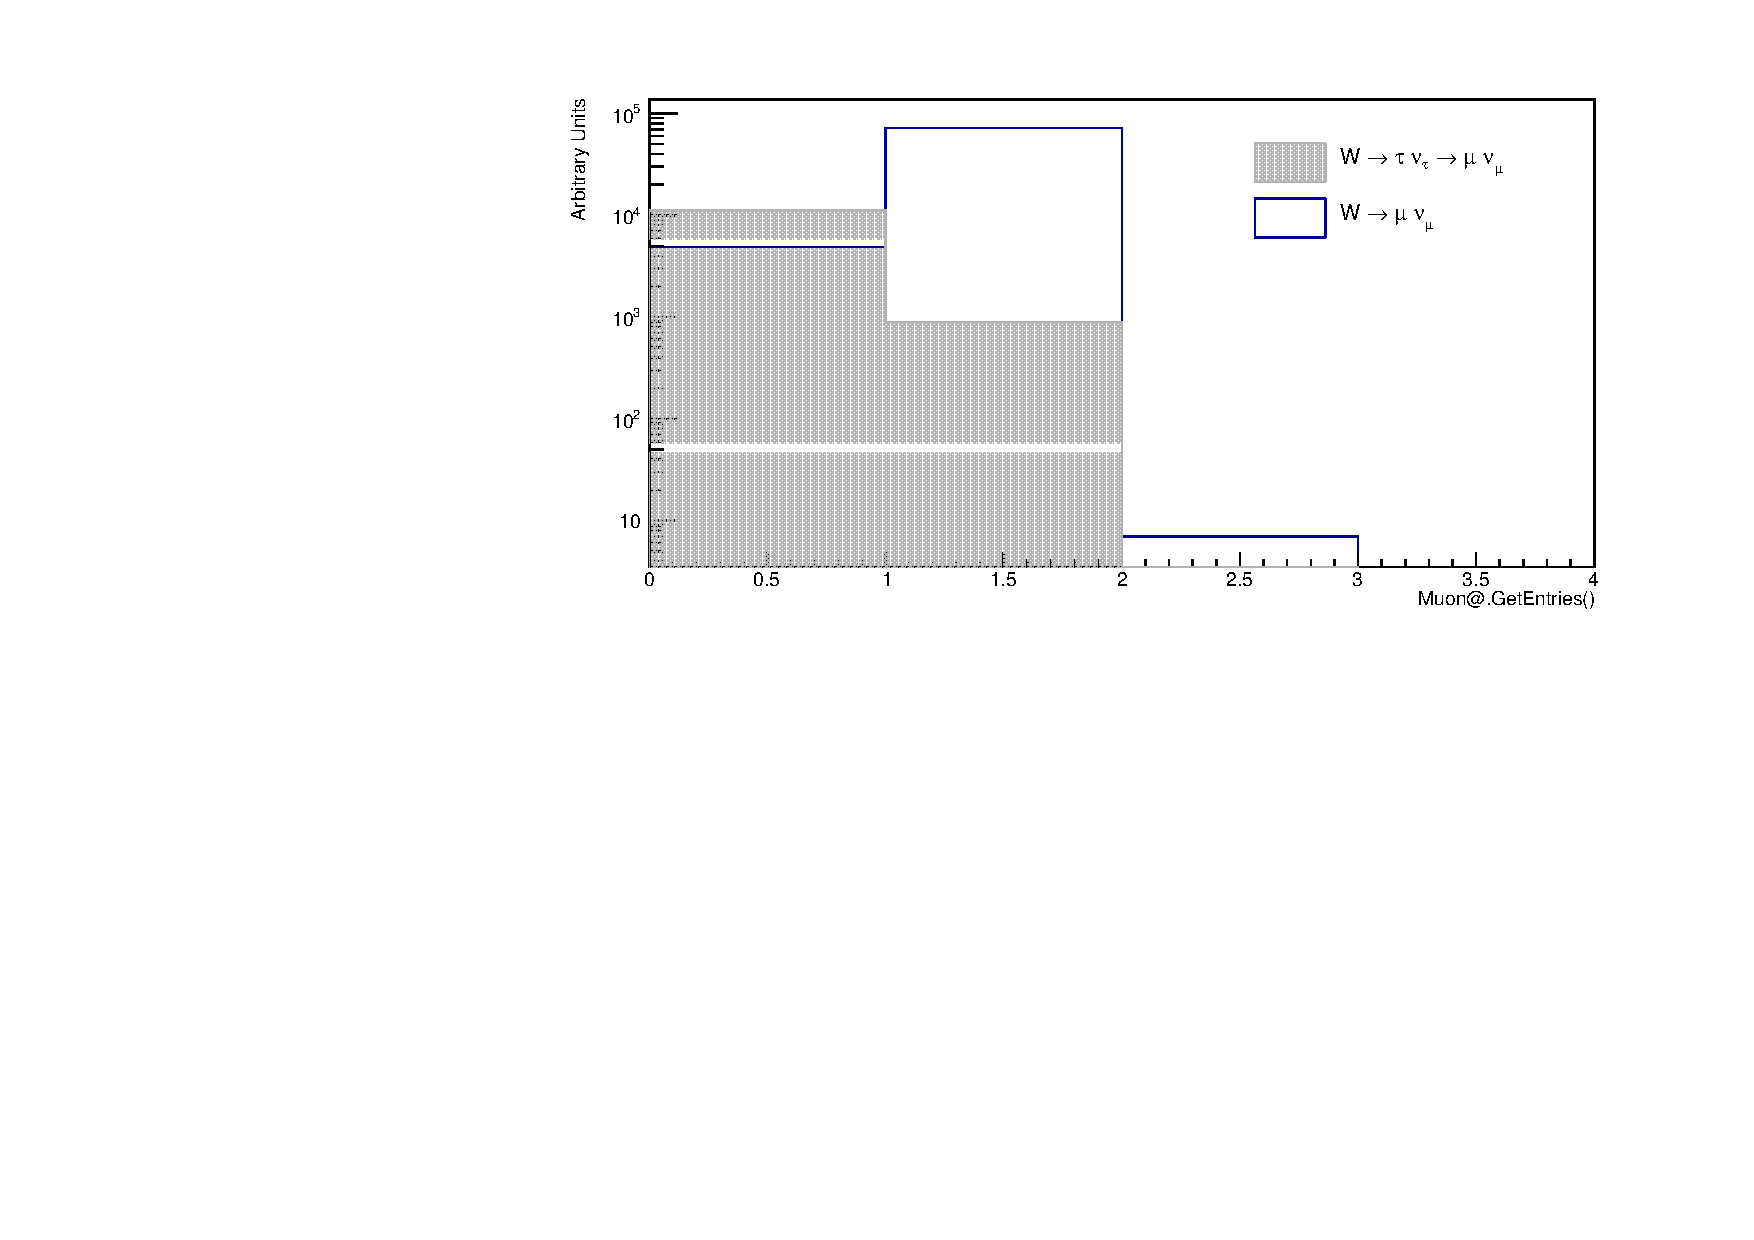
\includegraphics[width=1.0\textwidth]{pictures/MuonsSizeLog}\label{fig:f1}
	\caption{\scriptsize{ Numero de muones en el evento para los procesos $W \rightarrow \mu \nu_{\mu}$ y $W \rightarrow \tau \nu_{\tau} \rightarrow \mu \nu_{\mu}$}}
\end{figure}


\end{frame}

% ------------------------------------------------------------------------------------------------


%\section{Discución}

\begin{frame}
    \frametitle{Yields con las diferentes XS}
    
    
  	{\tiny
		    
	    \begin{table}[]
	    	\begin{tabular}{|l|l|l|l|l|}
	    		\hline
	    		\multicolumn{5}{|c|}{\textbf{W+Jets}}                                                                                                                                                            \\ \hline
	    		\textbf{}                                           & \textbf{W-\textgreater{}mu nu} & \textbf{W-\textgreater{}tau nu} & \textbf{W-\textgreater{}l nu} & \textbf{W-\textgreater{}mu nu (old XS)} \\ \hline
	    		\textbf{XSection (Pb)}                              & 940.61                         & 933.80                          & 2,833.06                      & 3,091.50                                \\ \hline
	    		\textbf{Esperados (100fb-1)}                        & 94,061,400.00                  & 93,380,000.00                   & 283,306,000.00                & 309,150,000.00                          \\ \hline
	    		\textbf{Montecarlo}                                 & 12,085.00                      & 12,024.00                       & 12,124.00                     & 4,031,811.00                            \\ \hline
	    		\textbf{MuonSize}                                   & 7,223.00                       & 897.00                          & 2,699.00                      & -                                       \\ \hline
	    		\textbf{MET\textgreater{}110, MHT\textgreater{}110} & 363.00                         & 92.00                           & 160.00                        & -                                       \\ \hline
	    		\textbf{MuonSize==1}                                & 363.00                         & 92.00                           & 160.00                        & -                                       \\ \hline
	    		\textbf{All}                                        & 18.00                          & 26.00                           & 17.00                         & 6,932.00                                \\ \hline
	    		\textbf{Peso}                                       & 7,783.32                       & 7,766.13                        & 23,367.37                     & 76.68                                   \\ \hline
	    		\textbf{Final Pesado}                               & 140,099.73                     & 201,919.49                      & 397,245.30                    & 531,529.83                              \\ \hline
	    	\end{tabular}
    	\caption{Eventos para diferentes secciones eficaces}
	    \end{table}
	    
    }
\end{frame}


% ----------------------------------------------------------------


% ------------------------------------------------------------------------------------------------

\ThankYouFrame

% ------------------------------------------------------------------------------------------------

\end{document}
